\documentclass{scrartcl}

\usepackage{fullpage}
\usepackage[utf8]{inputenc}
\usepackage{amsmath}
\usepackage{amssymb}
\usepackage{amsthm}
\usepackage{hyperref}
\usepackage{float}
\usepackage{verbatim}
\usepackage{color}
\usepackage{tikz}
\usetikzlibrary{positioning, shapes, arrows}

\newtheorem{mydef}{Definition}
\newtheorem{remark}{Remark}

\title{Report Generator}
\subtitle{module for otu.lea}
\author{Tamás Nagy\\ \small nattomi@gmail.com}

\begin{document}
\maketitle
\tableofcontents
\section{Introduction}
\href{http://github.com/nattomi/otulear}{Report Generator} is a module of the more complex \href{http://workforce.zmml.uni-bremen.de}{otu.lea} project. It is used for generating plain text and pdf reports about the performance of the users of the main \href{http://www.ifeb.uni-bremen.de/otulea/reaApplication.html}{otulea} test-taking application. It is a collection of \href{http://github.com/nattomi/otulear/tree/master/scripts}{scripts} (written in R and PHP) and \LaTeX\ templates. Additionally, routines used in the above mentioned scripts are also wrapped into an \href{http://github.com/nattomi/otulear/tree/master/otulea}{R package}. Momentarily it is not clear weather the R package is of any use, so its develepment is inactive. 

\section{How report generation works?}
Report generation is a process consisting of the following steps:
\begin{enumerate}
\item Load content of input data sources (such as .xml files) into memory
\item Extract information to be reported
\item\label{organ} Organize information to be reported into a structured form (such as .xml or .tex files)
\item If needed, run an external program (such as pdflatex) to translate the output of \ref{organ} into a human-readable form. 
\end{enumerate}
\begin{figure}[t]
\begin{center}
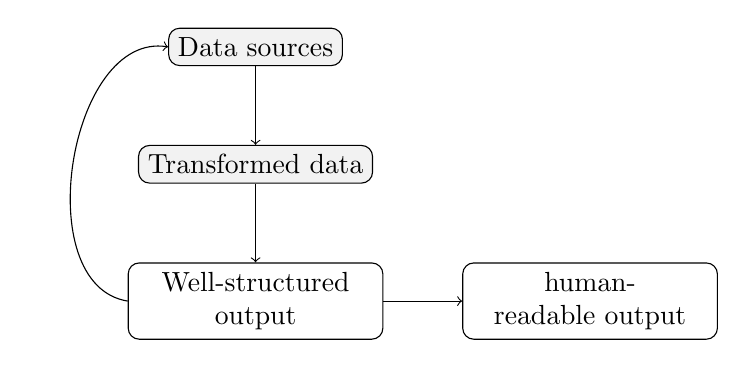
\begin{tikzpicture}[
mynode/.style={draw,fill=gray!10,rounded corners,align=center},
output/.style={draw,rounded corners,align=center}
]
\node[mynode] (sources) at (0,0) {Data sources};
\node[mynode, below=of sources] (trans) {Transformed data};
\node[output, below=of trans,text width=3cm] (struct) {Well-structured output};
\node[output,right=of struct,text width=3cm] (human) {human-readable output};
\draw[->] (sources) -- (trans);
\draw[->] (trans) -- (struct);
\draw[->] (struct) -- (human);
\path[->] (struct) edge [bend left=90] (sources);
\end{tikzpicture}
\end{center}
\caption{Simplified flow chart of report generation. It might be the case that a well-structured output of the report generation process becomes an input data source in a later stage.
}
\end{figure}
As an example, let's consider a speacial way to interpret the data generated by users of the otu.lea system, the so-called \emph{student report}. Here, we load certain .xml files, do some calculations on them according to some rules and dump the results of our calculations as an .xml file again. This .xml file becomes the input of a new calculation stream which outputs a .tex file. This file is then rendered into a pdf file using pdflatex. We talk about this later in more detail.

In general, we can say that there is always some sort of database (either a relational one our a database of static files in a well-organized folder hierarchy just like in the case of otu.lea) we get our data from. We can think of report generation as if it were a certain \emph{view} to our database -- similar to the concept under the same name in database theory.

\section{The otu.lea database}
The database behind the otu.lea system is a collection of static .xml files. There are two main parts of this database. Files in the first part are for configuration purposes that only administrators can modify. From these, Report Generator only uses one file named \emph{alphalist.xml}. Files in the other part of the database are generated while users of the system are taking test-sessions. We use the term \emph{user files} to describe them.
\subsection{The alphalist.xml file}
\begin{figure}
\begin{center}
\begin{tikzpicture}[
mynode/.style={draw,fill=gray!10,rounded corners,align=center},
output/.style={draw,rounded corners,align=center,anchor=north}
]
\node[mynode] (root) at (0,0) {alphalist};
\node[output,anchor=north] (a1) at (-5,-1) {\parbox{2.6cm}{\textbf{alphanode}\\
\small{$\bullet$ alphaID\\
$\bullet$ order\\
$\bullet$ description\\
$\bullet$ userdescription\\
$\bullet$ example}}};
\node[output] (a2) at (-.5,-1) {\textbf{alphanode}};
\node[anchor=north] (a3) at (1.25,-1.1) {$\ldots$};
\node[output] (a4) at (3,-1) {\textbf{alphanode}};
\draw[--] (root) -- (a1);
\draw[--] (root) -- (a2);
\draw[--] (root) -- (a4);
\end{tikzpicture}
\end{center}
\caption{Tree structure of the alphalist.xml file. Each alphanode entry has 5 attributes.}
\label{fig:alphalist}
\end{figure}
The structure of the file is explained in Figure \ref{fig:alphalist}. It consists of multiple alphanode nodes. Each alphanode node has 5 attributes:
\begin{description}
\item[alphaID]: ability description ID.
\item[order]: unrelevant for Report Generator.
\item[description]: ability description displayed for teachers
\item[userdescription]: ability description displayed for students 
\item[example]: example clarifying ability description (to be shown to students)
\end{description}
Here is a snippet from the file:
\begin{verbatim}
<alphalist lang="german">
  <alphanode alphaID="1.2.1.2" order="60"
             description="Kann Zeitpläne sinnentnehmend lesen" 
             userdescription="Ich kann Zeitpläne lesen" example=""/>
 <alphanode alphaID="1.2.1.1" order="50" 
            description="Kann Wörter mit ansteigender Komplexität 
                        (Konsonantenhäufung) recodieren und decodieren" 
            userdescription="Ich kann einfache Wörter erkennen und lesen" 
            example=""/>
\end{verbatim}
\quad$\vdots$
\subsection{The user files}\label{subsection:userfiles}
There are two type of users of the otu.lea system: teachers and students. In this document -- if not otherwise stated -- by the term user we always mean students. Each user has an id which is a character string of a fixed length. Let's denote it by \verb+$userid+. Each user has a folder in the database named as \verb+$userid+. In each folder, there is a special file named \verb+$userid . ".xml"+ (we use the operator . for string concatenation as in PHP). This file describes the tests taken by the user, we call it the \emph{global user file}. It serves as a search index for finding the information related to any particular test a user has taken. From it we can determine:
\begin{itemize}
\item The date and time a partical test session was started
\item The subject and level of this particular test
\item The tasks contained by this particular test and the \emph{task-result files} linked to them
\end{itemize}
\begin{figure}
\begin{center}
\begin{tikzpicture}[
mynode/.style={draw,fill=gray!10,rounded corners,align=center},
output/.style={draw,rounded corners,align=center,anchor=north}
]
\node[mynode] (root) at (0,0) {performedtests};
\node[output,anchor=north] (a1) at (-5,-1) {\parbox{2.6cm}{\textbf{test}\\
\small{$\bullet$ timestamp\\
$\bullet$ subject\\
$\bullet$ level}}};
\node[output] (a2) at (-.5,-1) {\textbf{test}};
\node[anchor=north] (a3) at (1.25,-1.1) {$\ldots$};
\node[output] (a4) at (3,-1) {\textbf{test}};
\draw[--] (root) -- (a1);
\draw[--] (root) -- (a2);
\draw[--] (root) -- (a4);
\node[output,anchor=north] (i1) at (-10,-4) {\parbox{2.6cm}{\textbf{item}\\
\small{$\bullet$ iname\\
$\bullet$ data}}};
\node[output] (i2) at (-5.5,-4) {\textbf{item}};
\node[anchor=north] (i3) at (-3.75,-4.1) {$\ldots$};
\node[output] (i4) at (-2,-4) {\textbf{item}};
\draw[--] (a1) -- (i1);
\draw[--] (a1) -- (i2);
\draw[--] (a1) -- (i4);
\end{tikzpicture}
\end{center}
\caption{Tree structure of the global user file. It contains information about the performed tests and the tasks within those tests.}
\label{fig:guf}
\end{figure}
Figure \ref{fig:guf} shows the tree structure of the global user file. The main document consists of various \emph{test} nodes. Each test node has the follwing attributes:
\begin{description}
\item[timestamp] character string describing the date and time of the beginning of the test-session in the form of \verb+%Y_%m_%d_%H_%M_%S+ (see Appendix \ref{app:posix} for notation).
\item[subject] character string describing the subject of the test. It can be one of ``Lesen'', ``Schreiben'', ``Sprache'', ``Mathe''.
\item[level] character string describing the difficulty of the test. It can be one of ``Einfach'', ``Mittel'' and ``Schwer''. 
\end{description}
\begin{remark}
I must extend this list with the newly implemented attribute \emph{prev}.
\end{remark}
Furthermore, each test node has child nodes called \emph{item}. The attributes of each of these item nodes are in one-to-one correspondence with a task of the test the parent node referring to. It has the following attributes:
\begin{description}
\item[iname] character string describing the number of the task. The numbering convention of the tasks is not detailed here.
\item[data] character string describing the name of the task-result file. The task-result files of a user are located in the same folder as the global user file. 
\end{description}
Below is a snippet from a global user file:
\begin{verbatim}  
<performedtests>
  <test timestamp="2014_2_27_12_40_49" subject="Schreiben" level="Einfach">
    <item iname="2.1.01" data="KFCG1_2014_2_27_12_40_49_2.1.01.xml"/>
    <item iname="2.1.02_I" data="KFCG1_2014_2_27_12_43_37_2.1.02_I.xml"/>
    <item iname="2.1.02_II" data="KFCG1_2014_2_27_12_47_9_2.1.02_II.xml"/>
    <item iname="2.2.01_III" data="KFCG1_2014_2_27_12_48_53_2.2.01_III.xml"/>
    <item iname="2.2.02_I" data="KFCG1_2014_2_27_12_52_11_2.2.02_I.xml"/>
  </test>
  <test timestamp="2014_2_27_18_37_23" subject="Lesen" level="Mittel">
    <item iname="1.3.2" data="KFCG1_2014_2_27_18_37_23_1.3.2.xml"/>
    <item iname="1.3.3" data="KFCG1_2014_2_27_18_40_45_1.3.3.xml"/>
    <item iname="1.3.4" data="KFCG1_2014_2_27_18_42_27_1.3.4.xml"/>
    <item iname="1.3.6" data="KFCG1_2014_2_27_18_43_53_1.3.6.xml"/>
    <item iname="1.4.1" data="KFCG1_2014_2_27_19_11_28_1.4.1.xml"/>
    <item iname="1.4.2" data="KFCG1_2014_2_27_19_14_19_1.4.2.xml"/>
    <item iname="1.4.4" data="KFCG1_2014_2_27_19_18_7_1.4.4.xml"/>
    <item iname="1.4.5" data="KFCG1_2014_2_27_19_22_52_1.4.5.xml"/>
    <item iname="1.4.6" data="KFCG1_2014_2_27_19_25_18_1.4.6.xml"/>
    <item iname="1.4.7" data="KFCG1_2014_2_27_19_27_16_1.4.7.xml"/>
    <item iname="1.4.8" data="KFCG1_2014_2_27_19_29_40_1.4.8.xml"/>
  </test>
\end{verbatim}
\quad$\vdots$

The structure of the task-result files are more diverse, but as Report Generator only uses a specific segment of the file, we intruduce only this segment in Figure \ref{fig:taskresult}.
\begin{figure}
\begin{center}
\begin{tikzpicture}[
mynode/.style={draw,fill=gray!10,rounded corners,align=center},
output/.style={draw,rounded corners,align=center,anchor=north}
]
\node[mynode] (root) at (0,0) {item};
\node[output] (marking) at (0,-1) {marking};
\node[output] (pointuse) at (-7,-2.5) {pointuse};
\node[output] (m1) at (-3.5,-2.5) {\parbox{2.6cm}{\textbf{mark}\\
\small{$\bullet$ itemnumber\\
$\bullet$ alphalevel}}};
\node[output] (m2) at (-.5,-2.5) {\textbf{mark}};
\node at (.75,-2.75) {$\ldots$};
\node[output] (m3) at (2,-2.5) {\textbf{mark}};
\draw[--] (root) -- (marking);
\draw[--] (marking) -- (pointuse);
\draw[--] (marking) -- (m1);
\draw[--] (marking) -- (m2);
\draw[--] (marking) -- (m3);
\end{tikzpicture}
\end{center}
\caption{Tree structure of the segment of the task-result file relevant to Report Generator.}
\label{fig:taskresult}
\end{figure}
In the task-result files there is always a \emph{marking} node whose children nodes we are interested in. It always has a child node named \emph{pointuse} which is not relevant to our calculations so we omit describing it. Its other children nodes are all named \emph{mark} and they describe the performance of the user on a subtask of the task in question. Performance can be either 1 (passed) or 0 (failed). Each mark node has (at least) the following attributes:
\begin{description}
\item[itemnumber] character string describing the subtask number the mark node is referring to
\item[alphalevel] ability description id of the ability description which is tested by the mark node
\end{description} 
Below is the simplified version of a the task-result file showing only the nodes relevant to Report Generator.
\begin{verbatim}
<item>
  <marking>
    <pointuse maxpoint="1"/>
    <mark itemnumber="2.1.01_1a" alphalevel="2.1.05">1</mark>
    <mark itemnumber="2.1.01_1b" alphalevel="2.1.14">1</mark>
    <mark itemnumber="2.1.01_2a" alphalevel="2.1.05">1</mark>
    <mark itemnumber="2.1.01_2b" alphalevel="2.1.14">1</mark>
    <mark itemnumber="2.1.01_3a" alphalevel="2.1.05">1</mark>
    <mark itemnumber="2.1.01_3b" alphalevel="2.1.04">1</mark>
    <mark itemnumber="2.1.01_4a" alphalevel="2.1.05">1</mark>
    <mark itemnumber="2.1.01_4b" alphalevel="2.1.14">1</mark>
    <mark itemnumber="2.1.01_5a" alphalevel="2.1.05">1</mark>
    <mark itemnumber="2.1.01_5b" alphalevel="2.1.14">0</mark>
    <mark itemnumber="2.1.01_5c" alphalevel="2.1.14">0</mark>
  </marking>
</item>
\end{verbatim}

\section{A first look at mark tables}\label{sec:intro}
\begin{remark}
This is the point where the separate document (eval.tex) was glued to the original manual (i.e. this document). There should be a section about how we get mark tables from our input data. The rest of the document assumes that we already obtained mark tables somehow.
\end{remark}

The performance of a user during a test-session (regardless whether the test was interrupted or not) can be summarized in a so-called \emph{mark table}. The formal definition of a mark table will be given later below, for now we just give an example for clarity:

\vspace{.5cm}
\begin{tabular}{lllllll}
timestamp	& subject	& level	& task	& subtask	& alphaid	& mark\\
2014\_11\_8\_10\_6\_59	& Schreiben	& Einfach	& 2.2.02\_III	& 2.2.02\_III\_10b	& 2.1.13	& 1\\
2014\_11\_8\_10\_6\_59	& Schreiben	& Einfach	& 2.2.02\_III	& 2.2.02\_III\_10c	& 2.1.08	& 1\\
2014\_11\_8\_10\_6\_59	& Schreiben	& Einfach	& 2.2.02\_III	& 2.2.02\_III\_11	& 2.2.08	& 0\\
2014\_11\_8\_10\_6\_59	& Schreiben	& Einfach	& 2.2.02\_III	& 2.2.02\_III\_12	& 2.2.08	& 1\\
2014\_11\_8\_10\_6\_59	& Schreiben	& Einfach	& 2.2.02\_III	& 2.2.02\_III\_13	& 2.1.07	& 0\\
2014\_11\_8\_9\_58\_0	& Schreiben	& Einfach	& 2.1.01	& 2.1.01\_1a	& 2.1.05	& 1\\
2014\_11\_8\_9\_58\_0	& Schreiben	& Einfach	& 2.1.01	& 2.1.01\_1b	& 2.1.14	& 1\\
2014\_11\_8\_9\_58\_0	& Schreiben	& Einfach	& 2.1.01	& 2.1.01\_2a	& 2.1.05	& 0\\
2014\_11\_8\_9\_58\_0	& Schreiben	& Einfach	& 2.1.01	& 2.1.01\_2b	& 2.1.14	& 0\\
\end{tabular}

\section{Definitions of some sets of concern}

Throughout this document the sets of some symbols are going to be referred to as a \emph{alphabet}. Some examples of a alphabet includes
$$\Delta^+=\{1,2,3,4,5,6,7,8,9\} \mbox{ and }\Delta=\{0\}\cup\Delta^+$$
which are going to be referred to as \emph{positive digits} and \emph{digits}, respectively. Another example is the set 
\begin{equation}
\begin{split}
\Omega=\Delta \cup \{.,\_\}\cup\{a,b,c,d,e,f,g,h,i,j,k,l,m,n,o,p,q,r,s,t,u,v,w,x,y,z,ä,ö,ü,ß\} & \cup\\
\{A,B,C,D,E,F,G,H,I,J,K,L,M,N,O,P,Q,R,S,T,U,V,W,X,Y,Z,Ä,Ö,Ü\}. & \\
\end{split}
\end{equation}
In this document when we use the word alphabet -- if not otherwise stated -- we always think about the set $\Omega$. It is trivial from the construction of the sets above that $\Delta^+\subset\Delta\subset\Omega$ and $\Delta^+\subset\Delta\subset\mathbb{N}$ where $\mathbb{N}$ denotes the set of natural numbers (including 0).

\begin{remark}
The last statement is not 100\% correct here because elements of $\Delta$ are just symbols not actual numbers, but we allow us this slight incorrectness because our notation is chosen so that it is clear that f.i. the digit $9\in\Delta$ symbolizes the number $9\in\mathbb{N}$.
\end{remark}
 
\begin{mydef}
Elements of the set $$\mathcal{W}_n(\Omega)=\underbrace{\Omega\times \Omega\times\ldots \times \Omega}_{n}$$ are called \emph{words of length n over the alphabet $\Omega$}. We define the \emph{set of words over the alphabet $\Omega$} as $$\mathcal{W}(\Omega)=\bigcup_{n=1}^{\infty}\mathcal{W}_n(\Omega).$$
\end{mydef}

\begin{mydef}
Let $w\in\mathcal{W}({\Omega})$. It is easy to prove that there exists a unique $n>0$ such that $w\in\mathcal{W}_n({\Omega})$. $n$ is called the \emph{length} of the word $w$ and it is denoted by $|w|$.
\end{mydef}

\begin{mydef} 
Elements of the set
$$\mathcal{I}=\mathcal{W}(\Delta)$$
are called \emph{integer words} whereas elements of the set
$$\mathcal{I}^+=\mathcal{I}\setminus\mathcal{W}(\{0\})$$ are called \emph{positive integer words}.
\end{mydef}

Some examples of integer words are $(1,0)$, $(1,0,2)$ or $(0,0,1,2)$. It is obvious that integer words got their name from the fact that they symbolize integer numbers, for instance
\begin{equation}
\begin{split}
(1,0)\mapsto & 10^0\cdot 0+10^1\cdot 1=10\\
(1,0,2)\mapsto & 10^0\cdot 2 + 10^1\cdot 0 + 10^2\cdot 1=102\\
(0,0,1,2)\mapsto & 10^0\cdot 2 + 10^1\cdot 1 + 10^2\cdot 0 + 10^3\cdot 0=12
\end{split}
\end{equation}

\begin{mydef}
Let $w\in\mathcal{I}$ and let $n=|w|$. Then there exists $d_1,d_2,\ldots,d_n\in\Delta\subset\mathbb{N}$ such that $w=(d_1,d_2,\ldots,d_n)$. The number $$w^{\ast}=\sum_{i=0}^{n-1}10^id_{n-i}$$ is called the \emph{integer value} of $w$.
\end{mydef}

\begin{mydef}
Let $A,B\subset\mathcal{W}$ be arbitrary sets. We call the set 
$$A.B=A\times\{.\}\times B\subset\mathcal{W}$$
the \emph{dotproduct} of those sets.
\end{mydef}

In the upcoming subsections we define some special subsets of $\mathcal{W}$.

\subsection{$\mathcal{T}$ - the set of timestamps}
I will give an exact definition later, for now it is enough to know that $\mathcal{T}\subset\mathcal{W}$.
\subsection{$\mathcal{S}$ - the set of subjects}
\begin{mydef}
The \emph{set of subjects} is defined as
\begin{equation}
\mathcal{S}=\{(L,e,s,e,n),(S,c,h,r,e,i,b,e,n),(S,c,h,p,r,a,c,h,e),(M,a,t,h,e)\}.
\end{equation}
\end{mydef}

\subsection{$\mathcal{L}$ - the set of levels}
\begin{mydef}
The \emph{set of levels} is defined as
\begin{equation}
\mathcal{L}=\{(E,i,n,f,a,c,h),(M,i,t,t,e,l),(S,c,h,w,e,r)\}.
\end{equation}
\end{mydef}

\subsection{$\mathcal{K}$ - the set of tasks}
I need more details in order to give an exact definition, for now it is enough to know that $\mathcal{K}\subset\mathcal{W}$.

\subsection{$\mathcal{U}$ - the set of subtasks}
I need more details in order to give an exact definition, for now it is enough to know that $\mathcal{U}\subset\mathcal{W}$.

\subsection{$\mathcal{A}$ - the set of alpha ids}
\begin{mydef}
Consider the following recursion of sets in $\mathcal{W}:$
\begin{equation}
\begin{split}
\mathcal{A}_0= & \mathcal{I}^+\\
\vdots &\\
\mathcal{A}_{n} = &\mathcal{A}_{n-1}.\mathcal{I}^+ \mbox{ for } n>1.\\
\end{split}
\end{equation}
The set $$\mathcal{A}=\bigcup_{n=0}^{\infty}\mathcal{A}_n\subset\mathcal{W}$$ is called the \emph{set of alpha ids}. 
\end{mydef}

Some examples of alpha ids are $(1,.,2,.,10)$, $(10,.,2)$ or $(1,.,2,.,0,2)$, but f.i.  $(10,.,0,.,9,.,10)$ or $(a,.,10,.,b)$ are not valid alpha ids. 

\begin{mydef}
For each $w\in\matchal{A}$ there exists a unique $n>0$ such that $w\in\mathcal{A}_n$. $n$ is called the dimension of $w$ and it is denoted by $\dim(w)$.
\end{mydef}

\begin{mydef}
Let $w\in\mathcal{A}$ and let $n=\dim(w)$. Then there exists $I_1,I_2,\ldots,I_n\in\mathcal{I}^+$ such that $w=(I_1,.,I_2,.,\ldots,.,I_n)$. The vector 
$$w^{\times}=(I_1^{\ast},I_2^{\ast},\ldots,I_n^{\ast})\in\mathbb{N}^n$$ is called the \emph{integer decomposition} of $w$.
\end{mydef}

It can be shown that one can define a total order on $\mathcal{A}$ using the following order relation.

\begin{mydef}
Let $\alpha, \beta\in\mathcal{A}$. We say that $\alpha\prec\beta$ if and only if
\begin{itemize}
\item there exists $0<m<\min(\dim\alpha,\dim\beta)$ such that $\alpha^{\times}_i=\beta^{\times}_i$ for all $i<m$ but $\alpha^{\times}_m<\beta^{\times}_m$ or
\item $\dim\alpha < \dim\beta$ and $\alpha^{\times}_i=\beta^{\times}_i$ for all $i\leq\dim\alpha$.
\end{itemize}
\end{mydef}

\section{A formal definition of mark tables}
Let $M=\{0,1\}$ and let us fix $\mathcal{F}\subset\mathcal{A}$, $|\mathcal{F}|<\infty$ as the set of \emph{feasible alpha ids}\footnote{This is an abstraction of the alpha ids in the \texttt{alphalist.xml} file}. We construct the set $\mu$ as 
$$\mu=\underbrace{\mathcal{T}}_{\mbox{timestamps}}\times\underbrace{\mathcal{S}}_{\mbox{subjects}}\times\underbrace{\mathcal{L}}_{\mbox{levels}}\times\underbrace{\mathcal{K}}_{\mbox{tasks}}\times\underbrace{\mathcal{U}}_{\mbox{subtasks}}\times\underbrace{\mathcal{F}}_{\mbox{alphaids}}\times \underbrace{B}_{\mbox{marks}}.$$ 
A \emph{mark table} is an element in $\mathcal{W}(\mathcal{\mu})$\footnote{I must emphasize earlier in the document that the notation $\mathcal{W}$ can be used not only for alphabets!}, but we can also think about it as a finite sequence $M=(m_i)_{i\in I}$ in $\mu$ with $I=\{1,2,\ldots,n\}$ for some $n<\infty$.

Before we go on we introduce some further notations related to finite, totally ordered sets.
\begin{mydef}
If $(R,\prec)$ is a finite, totally ordered set, then the sequence $R^{\prec}=(r^{\prec}_i)_{i=1}^{|R|}$ defined by the recursion
\begin{equation}
\begin{split}
r^{\prec}_1= & \min R\\
\vdots &\\
r^{\prec}_n = & \min R\setminus\{r^{\prec}_1,r^{\prec}_2,\ldots,r^{\prec}_{n-1}\} \mbox{ for } n>1.\\
\end{split}
\end{equation}
is called the \emph{increasing sequence} of $R$. Similarly, $R^{\succ}$ can be defined as the \emph{decreasing sequence}.
\end{mydef}

\section{Evaluation modes}
We present two different evaluation methods here, one is called ``Das kann ich!'' (\emph{mode A1}) and the other is called ``Das kann ich bald wenn ich moch ein wenig übe'' (\emph{mode A2}). The evaluation methods are basically mappings from $\mathcal{W}({\mathcal{M}})$ to the set of finite sequences over $\mathcal{F}$.

\subsection{Description of evaluation mode A1}
We start from a mark table $M=(m_i)_{i\in I}$. Let's define the relation $\sim$ over $I$ as follows:
\begin{equation}
i\sim j \Leftrightarrow m_i^{(6)}=m_j^{(6)}.
\label{eq:part}
\end{equation}
It is easy to see that (\ref{eq:part}) is an equivalence relation and as such it defines a partition over $I$, i.e. there exist some nonempty, disjoint sets $I_1,I_2,\ldots,I_r$ such that $$I=\cup_{i=1}^r I_i$$ and $i$ and $j$ are in $I_k$ if and only if $i\sim j$ i.e. $m_i^{(6)}=m_j^{(6)}$. Moreover, this resolution of $I$ is unique. Let us choose an element $i_k\in I_k$ (i.e. a \emph{representative}) for each $k=1,2,\ldots,r$.

Let $t\in [0,100]$ denote our predefined threshold for fullfilling a competency. Then, our preliminary result set is defined by 
$$R=\{m_{i_k}^{(6)}: |I_k|^{-1}\sum_{i \in I_k}m_{i}^{(7)}\geq 100^{-1}t, (k=1,2,\ldots r)\}.$$
Our final result is then $R^{\prec}$.
\begin{remark}
In our implementation we do not allow our result sequence to be longer then a predefined number $L\in\mathbb{N}^+$, so we take the sequence $(r^{\prec}_i)_{i=1}^{\min(|R|,L)}$ instead.    
\end{remark}

\begin{remark}
It is possible, that $R=\emptyset$, especially when the thresold $t$ is too high. In that case $R^{\prec}$ also becomes empty of course.
\end{remark}

\begin{remark}
Note that we could have projected or sequence into $\mathcal{F}\times\mathcal{B}$ because the other coordinates where not used at all in the evaluation.
\end{remark}
\subsection{Description of evaluation mode A2}
Assume that we have the marking table $M=(m_i)_{i\in I}$ in hand which is to be evaluated. At first We construct the set $I_0=\{i\in I: m_i^{(7)}=0\}\subset I$. Using the equivalence relation of \ref{eq:part} we can find nonempty, disjoint sets such that $$I_0=\cup_{i=1}^rI_i.$$ Let us choose an element $i_k\in I_k$ (i.e. a \emph{representative}) for each $k=1,2,\ldots,r$. Then, our preliminary result set is defined by
$$R=\{m^{(6)}_{i_k}:k=1,2,\ldots,r\}.$$
Our final result set is then $R^{\prec}$.
\begin{remark}
In our implementation we do not allow our result sequence to be longer then a predefined number $L\in\mathbb{N}^+$, so we take the sequence $(r^{\prec}_i)_{i=1}^{\min(|R|,L)}$ instead.    
\end{remark}
\begin{remark}
Note that we could have projected or sequence into $\mathcal{F}\times\mathcal{B}$ because the other coordinates where not used at all in the evaluation.
\end{remark}
\begin{remark}
If the mark received is 1 for each subtask, i.e. $m^{(7)}_i=1$ for all $i$ then $I_0=\emptyset$. In that case $R$ and consequently $R^{\prec}$ becomes empty too.
\end{remark}

\section{About XML result files}
There are two dimensions of evaluation: one lists ability description ids that the user already possesses (evaluation mode A1) and the other lists ability description ids that the user doesn't possess yet (evaluation mode A2). The result of the script is a xml document which is either printed to standard output or to a file. Figure \ref{fig:xmlstudent} shows the structure of the xml result file.
\begin{figure}
\begin{center}
\begin{tikzpicture}[
mynode/.style={draw,fill=gray!10,rounded corners,align=center},
output/.style={draw,rounded corners,align=center,anchor=north}
]
\node[mynode] (root) at (0,-1) {results};
\node[output] (print) at (-7,-2.5) {\parbox{2cm}{\textbf{print}\\
\small{$\bullet$ file}}};
\node[output] (timestamp) at (-3.5,-2.5) {\parbox{2.6cm}{\textbf{timestamp}\\
\small{$\bullet$ order\\
$\bullet$ value}}};
\node[output] (m2) at (-.5,-2.5) {\parbox{2cm}{\textbf{subject}\\
\small{$\bullet$ value}}};
\node[output] (m3) at (2,-2.5) {\parbox{2cm}{\textbf{level}\\
\small{$\bullet$ value}}};
\node[output,dashed] (m4) at (4.5,-2.5) {\parbox{2cm}{\textbf{eval}\\
\small{$\bullet$ mode}}};
\draw[--] (root) -- (print);
\draw[--] (root) -- (timestamp);
\draw[--] (root) -- (m2);
\draw[--] (root) -- (m3);
\draw[--] (root) -- (m4);
\node[output,dashed] (an1) at (-2,-5) {\parbox{2.6cm}{\textbf{alphanode}\\
\small{$\bullet$ alphaID\\
$\bullet$ userdescription\\
$\bullet$ example}}};
\node[output,dashed] (an2) at (1.5,-5) {\parbox{2.6cm}{\textbf{alphanode}}};
\node[output,dashed] (an3) at (6,-5) {\parbox{2.6cm}{\textbf{alphanode}}};
\node at (3.75,-5.25) {$\ldots$};
\draw[--] (m4) -- (an1);
\draw[--] (m4) -- (an2);
\draw[--] (m4) -- (an3)
\end{tikzpicture}
\end{center}
\caption{Tree structure of the xml document printed by evalUser.R. Depending on the actual input of the program nodes with a dashed border might not be present at all.}
\label{fig:xmlstudent}
\end{figure}
The following nodes are always present:
\begin{description}
\item[print] it has always one attribute called \emph{file}. The value of this attribute is identical to the value of the \verb+filename+ option concatenated with the string \verb+.pdf+. See also question \ref{q:xmlstructure}
\item[timestamp] it has 2 attributes. The first attribute, called \emp{order}, is always identical to \verb+YmdHis+. The second attribute, called \emph{value} is identical to the value of the \verb+xmltimestamp+ option.
\item[subject] it always has one attribute called \emph{value}. We always evaluate the performance of a certain user specified by the \verb+user+ option on a test specified by the \verb+timestamp+ option. The value is coming from the subject attribute of the relevant test node of this user's global user file. See also question \ref{q:xmlstructure}.
\item[level] it always has one attribute called \emph{value}. We always evaluate the performance of a certain user specified by the \verb+user+ option on a test specified by the \verb+timestamp+ option. The value is coming from the level attribute of the relevant test node of this user's global user file. See also question \ref{q:xmlstructure}.
\end{description}
On the other hand, \emph{eval} nodes are not always present, but if they are, they have an attribute named \emph{mode}. This attribute either has the value \emph{A1} or \emph{A2}. There are two possible options (we will discuss later in detail when these two cases arise):
\begin{enumerate}
\item No eval nodes exists at all.
\item There is one A1-type and one A2-type eval node.
\end{enumerate}
If eval nodes exists, they might (or might not) have children nodes named \emph{alphanode}. An A1-type eval node can not have more children node than the value of the option \verb+maxlistings+. An A2-type eval can not have more than 2 children node. The alphanode nodes have the following attributes:
\begin{description}
\item[alphaID] a certain ebility description id to be reported based on how the user performed on the test
\item[userdescription] user description belonging to the ability description id (taken from alphalist.xml) 
\item[example] example belonging to the ability description id (taken from alphalist.xml)
\end{description}

\appendix

\section{ISO C99 / POSIX standard for 'strftime'}\label{app:posix}
\begin{tabular}{rp{14cm}} 
\%d & Day of the month as decimal number (01-31).\\
\%H & Hours as decimal number (00-23).  As a special exception times such as ‘24:00:00’ are accepted for input, since ISO 8601 allows these.\\
\%m & Month as decimal number (01-12).\\
\%M & Minute as decimal number (00-59).\\
\%S & Second as decimal number (00-61), allowing for up to two leap-seconds (but POSIX-compliant implementations will ignore leap seconds).\\
\%Y & Year with century.  Note that whereas there was no zero in the original Gregorian calendar, ISO 8601:2004 defines it to be valid (interpreted as 1BC): see \url{http://en.wikipedia.org/wiki/0_(year)}.  Note that the standard also says that years before 1582 in its calendar should only be used with agreement of the parties involved.
\end{tabular}

\end{document}
